There are no established standard of characterisation measurements for granular materials. Common measurements include heap test, rotating drum test, linear/ring shear cell test, and the silo flow test,\ldots, in which the output is the bulk parameter, which defines how the granular material behaves in large quantity~-~such as angle of repose (AoR), shear stress, flow rate, etc. 

This research is focused on one of the most important bulk parameters to describe the characteristics of granular materials~-~the static angle of repose. Static AoR, which is described in Fig.~\ref{fig:StaticAoR}, is defined as the angle that granular solids forms when it piled with a flat surface, and is essential to characterise the coarseness and smootheness of materials. This in turn can help designing a process involved with the material~-~lower static AoR implies more flowable and thus easier to transport with less energy~\cite{TEFERRA201945}. 


\begin{figure}[t]
    \centering
    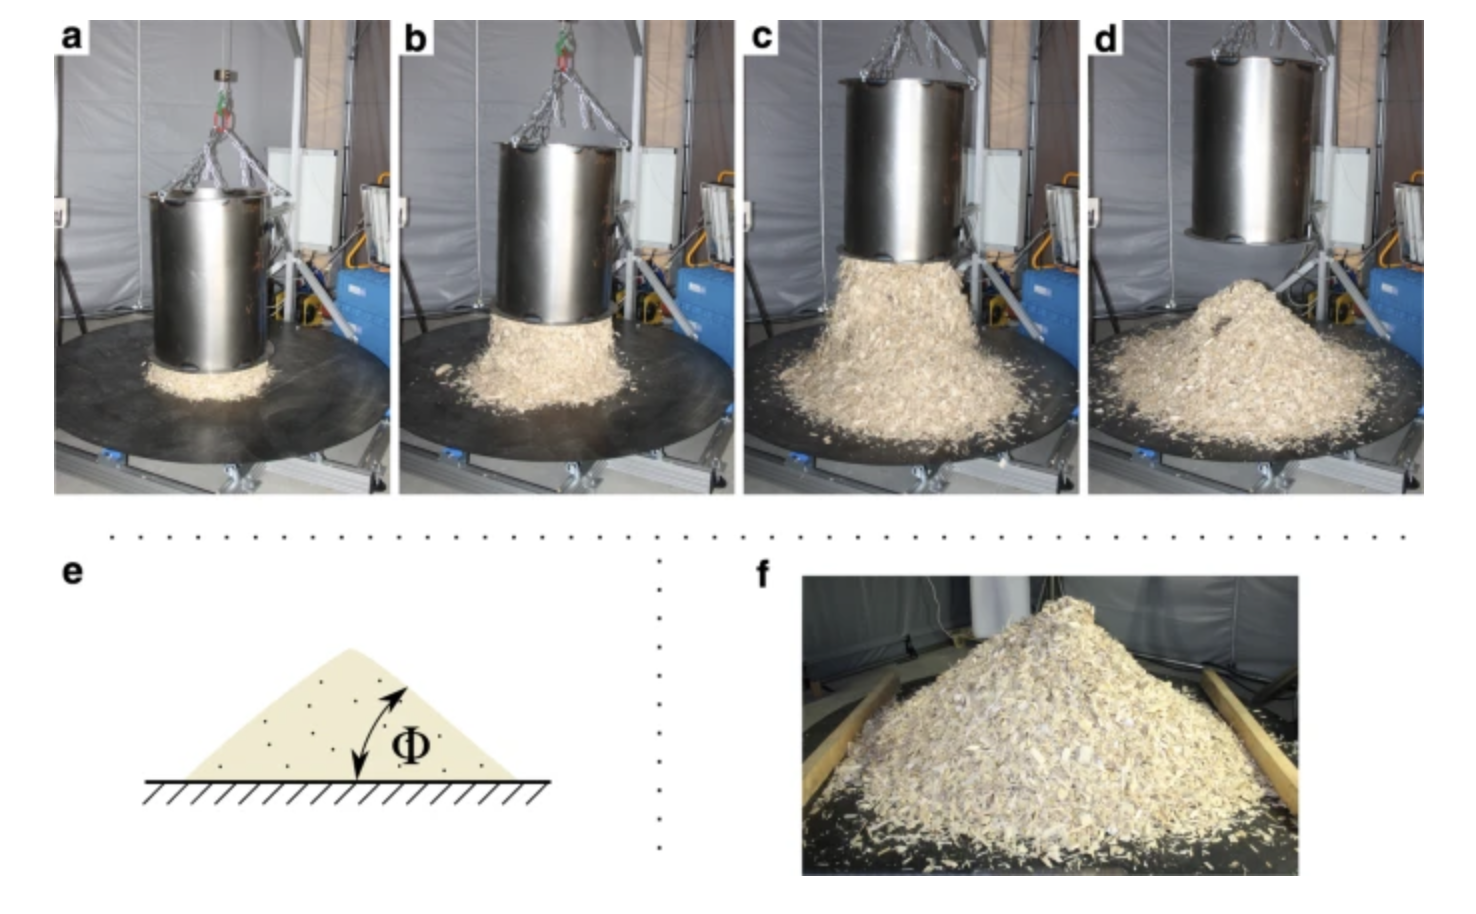
\includegraphics[scale=0.5]{StaticAoR.png}
    \caption{Static Angle of Repose measurement steps~\cite{Rackl:2018te}.}\label{fig:StaticAoR}
\end{figure}


